\documentclass[tikz]{standalone}
\usepackage{tikz}
\usetikzlibrary{backgrounds}

\begin{document}

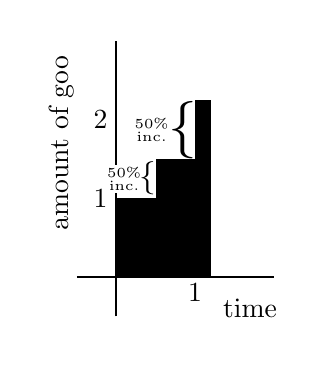
\begin{tikzpicture}[background rectangle/.style={fill=white}, show background rectangle]

% curve
\fill (0,1) -- (1,1) -- (1,0) -- (0,0);
\fill (0.5,0) -- (0.5,1.5) -- (1.1,1.5) -- (1.1,0);
\fill (1,0) -- (1,2.25) -- (1.2,2.25) -- (1.2, 0);

% axes
\draw[thick] (0,-0.5) -- (0,3);
\draw[thick] (-0.5,0) -- (2,0);
\draw[ultra thick, white] (0,1.06) -- (0,1.42);

% axes ticks
\path (-0.2, 1) node {1};
\path (-0.2, 2) node {2};
\path (1, -0.2) node {1};

% axes labels
\path (1.7, -0.4) node {time};
\path (-0.7, 1.7) node[rotate=90] {amount of goo};

% 50%
\path (0.4, 1.25) node {\large \{};
\path[align=center, text width=20pt] (0.1, 1.25) node {\tiny \baselineskip=1pt 50\% inc. \par};

\path (0.85, 1.87) node {\huge \{};
\path[align=center, text width=20pt] (0.45, 1.87) node {\tiny \baselineskip=1pt 50\% inc. \par};

\end{tikzpicture}

\end{document}




